\documentclass[10pt,letterpaper]{amspset}
\usepackage{fullpage}
\usepackage{gensymb}
\usepackage{graphicx}
\usepackage{tikz}
\usepackage{amsmath}
\graphicspath{ {./images/} }
\notag

% info for header block in upper right hand corner
\name{Brady Lamson}
\class{MATH 1120 SPRING 2021}
\assignment{Homework Part 2}
\duedate{Feb 7th}

\begin{document}

\problemlist{Unit Circle, Right Triangle and Trigonometric Functions Homework Assignment Part II:  

10.2 55-58, 65-70, 74

10.3 66—75, 77—80, 135, 137}

I will be repeatedly referencing the "Important Points of the Unit Circle" figure and a table of sine and cosine values. Both will be included in the reference section of this assignment. \bigskip
\hrule
\bigskip
In Exercises 55-58, find the measurement of the missing angle and the lengths of the missing sides.


\begin{problem}[55.]
Find $\theta, b, c.$

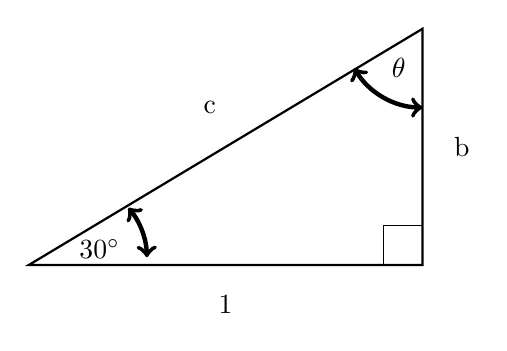
\begin{tikzpicture}
    \draw[black, thick] (0,0) -- (5,0) -- (5,3) -- cycle;
    \draw[ultra thick, <->] (1.5,.1) arc (1:40:1);
    \draw[ultra thick, <->] (5,2) arc (270:210:1);
    % Below nodes are the labels.
        \node[] at (0.9, 0.2) {$30\degree$};
        \node[] at (4.7, 2.5) {$\theta$};
        \node[] at (2.5, -0.5) {$1$};
        \node[] at (5.5, 1.5) {b};
        \node[] at (2.3, 2) {c};
    % This draws the right angle.
        \draw(4.5,0)|-(5,.5);
\end{tikzpicture}
\end{problem}

\begin{solution}[Solution]
The first thing we should do is figure out $\theta$. We know the sum of the angles for a trianle is 180\degree, so let's just do some basic arithmetic.  

\begin{align}
    \theta + 30\degree + 90\degree &= 180\degree \\
    \theta + 120\degree &= 180\degree
\end{align}
\[\boxed{ \theta = 60\degree }\]

From here we can use cosine to calculate the length of our hypotenuse. Remember, when it comes to triangles we know that $cos(\theta) = \frac{adjacent}{hypotenuse}$. I'll be using the $cos(30\degree)$, which we know to be $\frac{\sqrt{3}}{2}$.

\begin{align}
    cos(30\degree) &= \frac{1}{c} \\
    \frac{\sqrt{3}}{2} &= \frac{1}{c} \\
    c \cdot \left( \frac{\sqrt{3}}{2} \right) &= 1 \\
    c &= \left( \frac{1}{1} \right) \div \left( \frac{\sqrt{3}}{2} \right) \\
    c &= \left( \frac{1}{1} \right) \cdot \left( \frac{2}{\sqrt{3}} \right) \\
\end{align}

Now we need to get the $\sqrt{3}$ out of the denominator! 

\[c = \left( \frac{2}{\sqrt{3}} \right) \cdot \left( \frac{\sqrt{3}}{\sqrt{3}} \right)\]

\[\boxed{c = \frac{2 \sqrt{3}}{3}}\]

Okay that was really annoying, but now we're at the "easier" bit. We can use the pythagorean theorem, $a^2 + b^2 = c^2$ for the final side.

\begin{align}
    a &= 1 \\
    b &= b \\
    c &= \frac{2\sqrt{3}}{3}\\[+3mm]
    1^2 + b^2 &= \left( \frac{2\sqrt{3}}{3} \right) ^2 \\[+3mm]
    1^2 + b^2 &= \frac{4 \cdot 3}{9} \\[+3mm]
    b^2 &= \frac{12}{9} - \frac{9}{9} \\[+3mm]
    b^2 &= \frac{3}{9}
\end{align}

\[\boxed{ b = \frac{\sqrt{3}}{3}}\]

\end{solution}


\pagebreak


\begin{problem}[56.]
Find $\theta, a, c.$

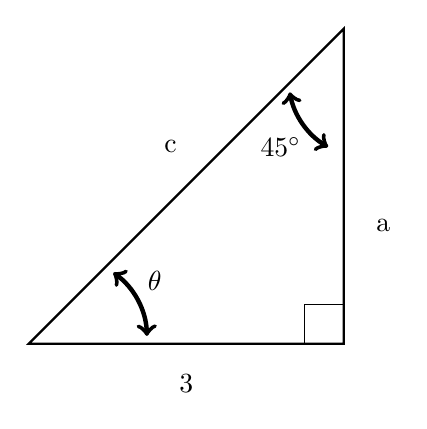
\begin{tikzpicture}
    \draw[black, thick] (0,0) -- (4,0) -- (4,4) -- cycle;
    % This draws the bottom left arc
        \draw[ultra thick, <->] (1.5,.1) arc (1:55:1);
    % This draws the top right arc, if you have any advice to making this guy better let me know!
        \draw[ultra thick, <->] (3.8,2.5) arc (240:190:1);
    % Below nodes are the labels.
        \node[] at (1.6, 0.8) {$\theta$};
        \node[] at (3.2, 2.5) {45\degree};
        \node[] at (2, -0.5) {$3$};
        \node[] at (4.5, 1.5) {a};
        \node[] at (1.8, 2.5) {c};
    % This draws the right angle.
        \draw(3.5,0)|-(4,.5);
\end{tikzpicture}
\end{problem}

\begin{solution}[Solution]
You know the drill, let's first solve for $\theta$.
\[90\degree = 45\degree + \theta\]
\[\boxed{\theta = 45\degree}\]

Solving for $a$ is deceptively simple. One truth of $45\degree$ right triangles is that the base and height are the same. This makes sense when you consider that this type of triangle is simply half of a square! So we can safely state the following.
\[b = 3\]
\[a = b\]
\[\boxed{a = 3}\]

Now we use the Pythagorean theorem to wrap this up.
\[a^2 + b^2 = c^2\]
\[3^2 + 3^2 = c^2\]
\[18 = c^2\]
\[c = \sqrt{3^2 \cdot 2}\]
\[\boxed{c = 3 \sqrt{2}}\]

\end{solution}


\pagebreak


\begin{problem}[57.]
Find $\alpha$, a and b.

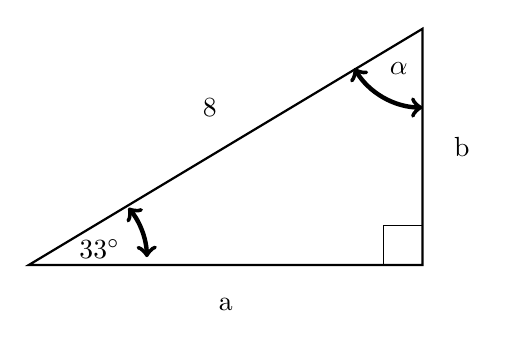
\begin{tikzpicture}
    \draw[black, thick] (0,0) -- (5,0) -- (5,3) -- cycle;
    \draw[ultra thick, <->] (1.5,.1) arc (1:40:1);
    \draw[ultra thick, <->] (5,2) arc (270:210:1);
    % Below nodes are the labels.
        \node[] at (0.9, 0.2) {$33\degree$};
        \node[] at (4.7, 2.5) {$\alpha$};
        \node[] at (2.5, -0.5) {a};
        \node[] at (5.5, 1.5) {b};
        \node[] at (2.3, 2) {8};
    % This draws the right angle.
        \draw(4.5,0)|-(5,.5);
\end{tikzpicture}
\end{problem}

\begin{solution}[Solution]
First we need to find $\alpha$, this is really easy as we can do the following.
\[\alpha + 33\degree = 90\degree\]
\[\boxed{\alpha = 57\degree}\]

\noindent  Here we can use the sine and cosine of $\alpha$ to find our two missing sides. Remember, $sin(\alpha) = \frac{opposite}{hypotenuse}$ and $cos(\alpha) = \frac{adjacent}{hypotenuse}$. 
\bigskip

Solving for a:
\[sin(57\degree) = \frac{a}{8} \]
\[\boxed{a = 8 \cdot sin(57\degree)}\]

\bigskip

Solving for b:
\[cos(57\degree) = \frac{b}{8}\]
\[\boxed{b = 8 \cdot cos(57\degree)}\]
\end{solution}


\pagebreak


\begin{problem}[58.]
Find $\beta$, a and c.

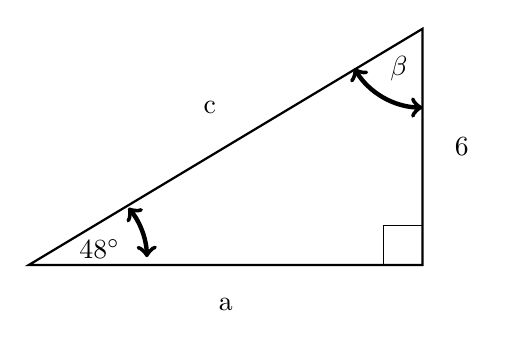
\begin{tikzpicture}
    \draw[black, thick] (0,0) -- (5,0) -- (5,3) -- cycle;
    \draw[ultra thick, <->] (1.5,.1) arc (1:40:1);
    \draw[ultra thick, <->] (5,2) arc (270:210:1);
    % Below nodes are the labels.
        \node[] at (0.9, 0.2) {$48\degree$};
        \node[] at (4.7, 2.5) {$\beta$};
        \node[] at (2.5, -0.5) {a};
        \node[] at (5.5, 1.5) {6};
        \node[] at (2.3, 2) {c};
    % This draws the right angle.
        \draw(4.5,0)|-(5,.5);
\end{tikzpicture}
\end{problem}

\begin{solution}[Solution]
First we need to find $\beta$.
\[\beta + 48\degree = 90\degree\]
\[\boxed{\beta = 42\degree}\]

\noindent  Here we can use the sine of our $48\degree$ angle and the tangent of $\beta$ to find our two missing sides. Remember, $sin(48\degree) = \frac{opposite}{hypotenuse}$ and $tan(\beta) = \frac{opposite}{adjacent}$. \bigskip

Solving for c:
\[sin(48\degree) = \frac{6}{c} \]
\[\boxed{c = \frac{6}{sin(48\degree)}}\]

\bigskip

Solving for a:
\[tan(42\degree) = \frac{a}{6}\]
\[\boxed{a = 6 \cdot tan(42\degree)}\]
\end{solution}


\pagebreak


In exercises 65-68, let $\theta$ be the angle in standard position whose terminal side contains the given
point then compute $cos(\theta)$ and $sin(\theta)$.

\begin{problem}[65.]
$P(-7, 24)$
\end{problem}

\begin{solution}[Solution]
This may seem a little unorthodox at first, but these problems become incredibly straightforward once you realize that the x and y coordinates are just another way to refer to the length and height of a right triangle! Let me show a representation of this.

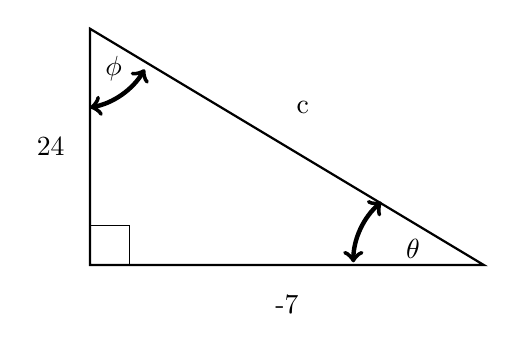
\begin{tikzpicture}
    \draw[black, thick] (0,0) -- (-5,0) -- (-5,3) -- cycle;
    \draw[ultra thick, <->] (-1.3,.8) arc (130:180:1);
    \draw[ultra thick, <->] (-5,2) arc (280:330:1);
    % Below nodes are the labels.
        \node[] at (-0.9, 0.2) {$\theta$};
        \node[] at (-4.7, 2.5) {$\phi$};
        \node[] at (-2.5, -0.5) {-7};
        \node[] at (-5.5, 1.5) {24};
        \node[] at (-2.3, 2) {c};
    % This draws the right angle.
        \draw(-4.5,0)|-(-5,.5);
\end{tikzpicture}

From here we really should solve for c, so we're going to do just that.
\begin{align}
    a^2 + b^2 &= c^2 \\
    -7^2 + 24^2 &= c^2 \\
    c^2 &= 49 + 576 \\
    c &= \sqrt{625} \\
    c &= 25
\end{align}

From here we just plug and chug. Though really we don't even need to chug in this case. Remember, $sin(\theta) = \frac{opposite}{hypotenuse}$ and $cos(\theta) = \frac{adjacent}{hypotenuse}$.

\[\boxed{cos(\theta) = - \frac{7}{25}}\]
\[\boxed{sin(\theta) = \frac{24}{25}}\]

\end{solution}


\pagebreak


\begin{problem}[66.]
$Q(3, 4)$
\end{problem}

\begin{solution}[Solution]
I'll be using the exact same logic and methodology as the previous problem here.
\bigskip

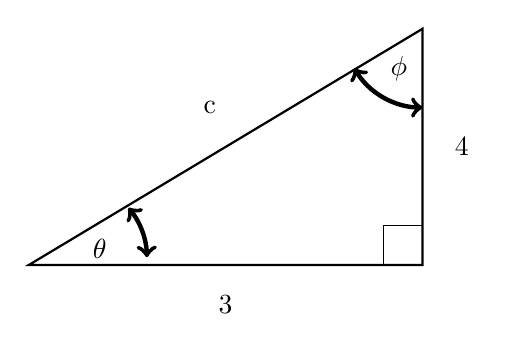
\begin{tikzpicture}
    \draw[black, thick] (0,0) -- (5,0) -- (5,3) -- cycle;
    \draw[ultra thick, <->] (1.5,.1) arc (1:40:1);
    \draw[ultra thick, <->] (5,2) arc (270:210:1);
    % Below nodes are the labels.
        \node[] at (0.9, 0.2) {$\theta$};
        \node[] at (4.7, 2.5) {$\phi$};
        \node[] at (2.5, -0.5) {3};
        \node[] at (5.5, 1.5) {4};
        \node[] at (2.3, 2) {c};
    % This draws the right angle.
        \draw(4.5,0)|-(5,.5);
\end{tikzpicture}

\bigskip

Solving for c.
\begin{align}
    c^2 &= a^2 + b^2 \\
    c^2 &= 3^2 + 4^2 \\
    c^2 &= 25 \\
    c &= 5 \\
\end{align}

Solving for cosine and sine of $\theta$. Remember, $sin(\theta) = \frac{opposite}{hypotenuse}$ and $cos(\theta) = \frac{adjacent}{hypotenuse}$.

\[\boxed{cos(\theta) = \frac{3}{5}}\]
\[\boxed{sin(\theta) = \frac{4}{5}}\]
\end{solution}


\pagebreak


\begin{problem}[67.]
$R(5, -9)$
\end{problem}

\begin{solution}[Solution]
I'll be using the exact same logic and methodology as the previous problems here. 
\bigskip

%This draws a triangle with a +x and -y
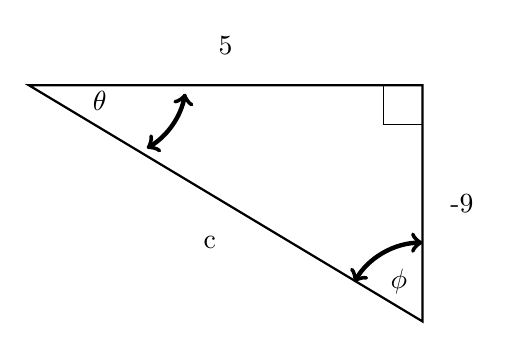
\begin{tikzpicture}
    \draw[black, thick] (0,0) -- (5,0) -- (5,-3) -- cycle;
    \draw[ultra thick, <->] (1.5,-.8) arc (300:350:1);
    \draw[ultra thick, <->] (5,-2.0) arc (90:150:1);
    % Below nodes are the labels.
        \node[] at (0.9, -0.2) {$\theta$};
        \node[] at (4.7, -2.5) {$\phi$};
        \node[] at (2.5, 0.5) {5};
        \node[] at (5.5, -1.5) {-9};
        \node[] at (2.3, -2) {c};
    % This draws the right angle.
        \draw(4.5,0)|-(5,-.5);
\end{tikzpicture}


Solving for c.
\begin{align}
c^2 &= a^2 + b^2 \\
c^2 &= 5^2 + -9^2 \\
c^2 &= 25 + 81 \\
c &= \sqrt{106} \\
\end{align}

Solving for sine and cosine of $\theta$. Remember, $sin(\theta) = \frac{opposite}{hypotenuse}$ and $cos(\theta) = \frac{adjacent}{hypotenuse}$.

\[\boxed{cos(\theta) = \frac{5}{\sqrt{106}}}\]
\[\boxed{sin(\theta) = -\frac{9}{\sqrt{106}}}\]
\end{solution}


\pagebreak


\begin{problem}[68.]
$T(-2, -11)$
\end{problem}

\begin{solution}[Solution]
I'll be using the exact same logic and methodology as the previous problems here. 
\bigskip

%This draws a triangle with a -x and -y
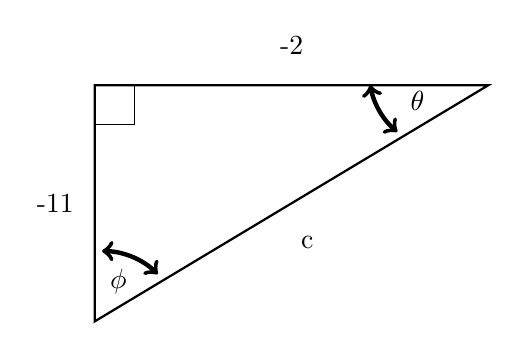
\begin{tikzpicture}
    \draw[black, thick] (0,0) -- (-5,0) -- (-5,-3) -- cycle;
    \draw[ultra thick, <->] (-1.5,0) arc (190:230:1);
    \draw[ultra thick, <->] (-4.2,-2.4) arc (45:90:1);
    % Below nodes are the labels.
        \node[] at (-0.9, -0.2) {$\theta$};
        \node[] at (-4.7, -2.5) {$\phi$};
        \node[] at (-2.5, 0.5) {-2};
        \node[] at (-5.5, -1.5) {-11};
        \node[] at (-2.3, -2) {c};
    % This draws the right angle.
        \draw(-4.5,0)|-(-5,-.5);
\end{tikzpicture}
\bigskip

Solving for c.
\begin{align}
    c^2 &= a^2 + b^2 \\
    c^2 &= -2^2 + -11^2 \\
    c^2 &= 4 + 121 \\
    c &= \sqrt{125} \\
    c &= 5\sqrt{5}
\end{align}

Solving for sine and cosine of $\theta$. Remember, $sin(\theta) = \frac{opposite}{hypotenuse}$ and $cos(\theta) = \frac{adjacent}{hypotenuse}$.

\[\boxed{cos(\theta) = -\frac{2}{5\sqrt{5}}}\]
\[\boxed{sin(\theta) = -\frac{11}{5\sqrt{5}}}\]
\end{solution}


\pagebreak


In Exercises 69 - 70, find the equations of motion for the given scenario. Assume that the center of
the motion is the origin, the motion is counter-clockwise and that t = 0 corresponds to a position
along the positive x-axis.

\begin{problem}[69.]
A point on the edge of the spinning yo-yo in Exercise 50 from Section 10.1.
Recall: The diameter of the yo-yo is 2.25 inches and it spins at 4500 revolutions per minute.
\end{problem}

\begin{solution}[Solution]

First be sure to always list off our givens.

\begin{align}
    d &= 2.25 inches \\
    r &= 1.125 inches \\
    \omega &= \frac{4500 \cdot 2\pi}{1 minute} \\
    \omega &= 9000\pi \frac{radians}{minute} \\
\end{align}

To solve this problem we can utilize Equation 10.3 from the textbook. 

\begin{problem}[Equation 10.3]
Suppose an object is traveling in a circular path of radius r centered at the origin with constant angular velocity $\omega$. If t = 0 corresponds to the point (r, 0), then the x and y coordinates of the object are functions of t and are given by $x = r \cdot cos(\omega \cdot t)$ and $y = r \cdot sin(\omega \cdot t)$. Here, $\omega > 0$ indicates a counter-clockwise direction and $\omega < 0$ indicates a clockwise direction.
\end{problem}

\bigskip

So, let's use the two equations provided by the textbook here! 
\[x = r \cdot cos(\omega \cdot t)\]
\[\boxed{x = 1.125 \cdot cos(9000\pi \cdot t)}\]
\[y = r \cdot sin(\omega \cdot t)\]
\[\boxed{y = 1.125 \cdot sin(9000\pi \cdot t)}\]
\footnote{Do note that r is in inches and t is in minutes.}

\end{solution}


\pagebreak


\begin{problem}[70]
The yo-yo in exercise 52 from Section 10.1.
Recall: The radius of the circle is 28 inches and it completes one revolution in 3 seconds.
\end{problem}

\begin{solution}[Solution]
Giving out the givens.
\begin{align}
    r &= 28 \\
    t &= 3 \\
    \omega &= \frac{2\pi}{3}
\end{align}

For the following logic please refer to problem 69.
\[x = r \cdot cos(\omega \cdot t)\]
\[\boxed{x = 28 \cdot cos\left( \frac{2\pi}{3} \cdot t \right)}\]
\[y = r \cdot sin(\omega \cdot t)\]
\[\boxed{y = 28 \cdot sin\left( \frac{2\pi}{3} \cdot t \right)}\]
\footnote{Do note that r is in inches and t is in seconds.}
\end{solution}


\pagebreak


\begin{problem}[74]
Let $\alpha$ and $\beta$ be the two acute angles of a right triangle. (Thus $\alpha$ and $\beta$ are complementary angles.) Show that $sin(\alpha) = cos(\beta)$ and $sin(\beta) = cos(\alpha)$.
\end{problem}

\begin{solution}[Solution]

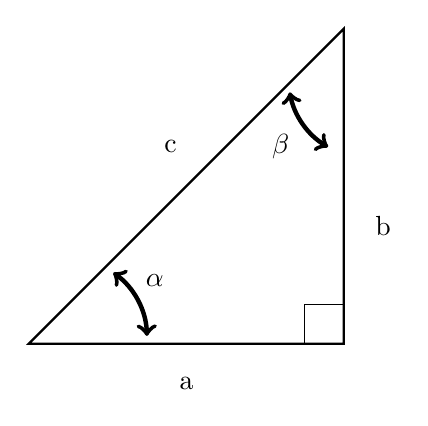
\begin{tikzpicture}
    \draw[black, thick] (0,0) -- (4,0) -- (4,4) -- cycle;
    % This draws the bottom left arc
        \draw[ultra thick, <->] (1.5,.1) arc (1:55:1);
    % This draws the top right arc, if you have any advice to making this guy better let me know!
        \draw[ultra thick, <->] (3.8,2.5) arc (240:190:1);
    % Below nodes are the labels.
        \node[] at (1.6, 0.8) {$\alpha$};
        \node[] at (3.2, 2.5) {$\beta$};
        \node[] at (2, -0.5) {a};
        \node[] at (4.5, 1.5) {b};
        \node[] at (1.8, 2.5) {c};
    % This draws the right angle.
        \draw(3.5,0)|-(4,.5);
\end{tikzpicture}

\bigskip

This is pretty easy to show when we utilize soh cah toa. We'll only need soh and cah for this problem. For those unfamiliar soh cah toa refers to the following rules regarding right triangles.

\[sin(\theta) = \frac{opposite}{hypotenuse}\]
\[cos(\theta) = \frac{adjacent}{hypotenuse}\]
\[tan(\theta) = \frac{opposite}{adjacent}\]

Thanks to these rules we can easily prove both.  
\bigskip

This proves the first statement.
\[sin(\alpha) = \frac{b}{c}\]
\[cos(\beta) = \frac{b}{c}\]
\[\boxed{sin(\alpha) = \cos(\beta)}\]

This proves the second statement.
\[sin(\beta) = \frac{a}{c}\]
\[cos(\alpha) = \frac{a}{c}\]
\[\boxed{sin(\beta) = \cos(\alpha)}\]
\end{solution}


\pagebreak

10.3 66—75, 77—80, 135, 137  

In Exercises 66-69, use Theorem 10.10 to find the requested quantities.

\begin{problem}[66]
Find $\theta$ a and c.
\end{problem}

\begin{solution}

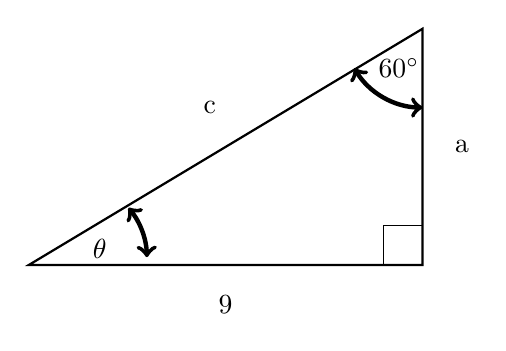
\begin{tikzpicture}
    \draw[black, thick] (0,0) -- (5,0) -- (5,3) -- cycle;
    \draw[ultra thick, <->] (1.5,.1) arc (1:40:1);
    \draw[ultra thick, <->] (5,2) arc (270:210:1);
    % Below nodes are the labels.
        \node[] at (0.9, 0.2) {$\theta$};
        \node[] at (4.7, 2.5) {60\degree};
        \node[] at (2.5, -0.5) {9};
        \node[] at (5.5, 1.5) {a};
        \node[] at (2.3, 2) {c};
    % This draws the right angle.
        \draw(4.5,0)|-(5,.5);
\end{tikzpicture}

First we calculate $\theta$.
\[\theta = 90\degree - 60\degree\]
\[\boxed{\theta = 30\degree}\]

Now we're going to do the arduous process of calculating a. I'll be using the tangent of the $60\degree$ angle which is thankfully a known value. We know that $tan(60\degree) = \sqrt{3}$. 

\begin{align}
    tan(60\degree) &= \frac{opposite}{adjacent} \\
    \sqrt{3} &= \frac{9}{a} \\
    a \cdot \sqrt{3} &= 9
\end{align}

\[a = \frac{9}{\sqrt{3}} = \frac{9 \cdot \sqrt{3}}{3}\]
\[\boxed{a = 3\sqrt{3}} \\\]

For the last side we'll just use the Pythagorean theorem. 

\begin{align}
a^2 + b^2 &= c^2 \\
(3\sqrt{3})^2 + 9^2 &= c^2 \\
27 + 81 &= c^2 \\
108 &= c^2 \\
\sqrt{108} &= c
\end{align}

\[\boxed{c = 6\sqrt{3}}\]

\end{solution}


\pagebreak


\begin{problem}[67]
Find $\theta$, b and c
\end{problem}

\begin{solution}

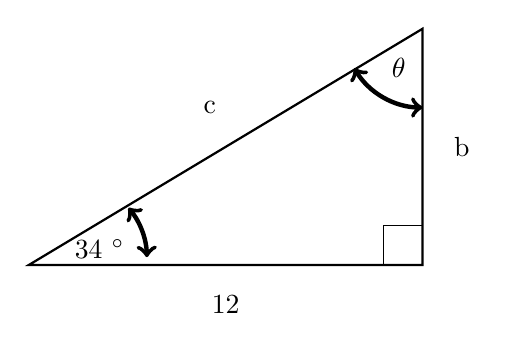
\begin{tikzpicture}
    \draw[black, thick] (0,0) -- (5,0) -- (5,3) -- cycle;
    \draw[ultra thick, <->] (1.5,.1) arc (1:40:1);
    \draw[ultra thick, <->] (5,2) arc (270:210:1);
    % Below nodes are the labels.
        \node[] at (0.9, 0.2) {34 \degree};
        \node[] at (4.7, 2.5) {$\theta$};
        \node[] at (2.5, -0.5) {12};
        \node[] at (5.5, 1.5) {b};
        \node[] at (2.3, 2) {c};
    % This draws the right angle.
        \draw(4.5,0)|-(5,.5);
\end{tikzpicture}

\[\theta = 90 - 34\]
\[\boxed{\theta = 56\degree}\]

To solve for c we will use secant and for b we will use tangent.

\[sec(34) = \frac{c}{12}\]
\[\boxed{c = 12 \cdot sec(34)}\]

\[tan(34) = \frac{b}{12}\]
\[\boxed{b = 12 \cdot tan(34)}\]

\end{solution}


\begin{problem}[68]
Find $\theta$, b and c.
\end{problem}

\begin{solution}
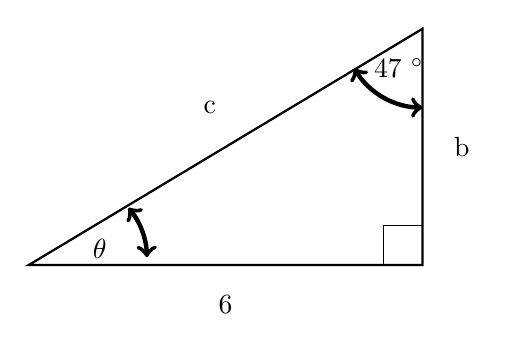
\begin{tikzpicture}
    \draw[black, thick] (0,0) -- (5,0) -- (5,3) -- cycle;
    \draw[ultra thick, <->] (1.5,.1) arc (1:40:1);
    \draw[ultra thick, <->] (5,2) arc (270:210:1);
    % Below nodes are the labels.
        \node[] at (0.9, 0.2) {$\theta$};
        \node[] at (4.7, 2.5) {47 \degree};
        \node[] at (2.5, -0.5) {6};
        \node[] at (5.5, 1.5) {b};
        \node[] at (2.3, 2) {c};
    % This draws the right angle.
        \draw(4.5,0)|-(5,.5);
\end{tikzpicture}

\[\theta = 90 - 47\]
\[\boxed{\theta = 43\degree}\]

\[tan(43) = \frac{a}{6}\]
\[\boxed{a = 6 \cdot tan(43)}\]

\[csc(47) = \frac{c}{6}\]
\[\boxed{c = 6 \cdot csc(47)}\]

\end{solution}


\begin{problem}[69]
Find $\theta$, b and c.
\end{problem}

\begin{solution}
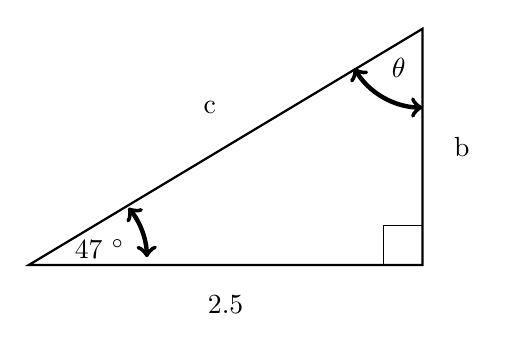
\begin{tikzpicture}
    \draw[black, thick] (0,0) -- (5,0) -- (5,3) -- cycle;
    \draw[ultra thick, <->] (1.5,.1) arc (1:40:1);
    \draw[ultra thick, <->] (5,2) arc (270:210:1);
    % Below nodes are the labels.
        \node[] at (0.9, 0.2) {47 \degree};
        \node[] at (4.7, 2.5) {$\theta$};
        \node[] at (2.5, -0.5) {2.5};
        \node[] at (5.5, 1.5) {b};
        \node[] at (2.3, 2) {c};
    % This draws the right angle.
        \draw(4.5,0)|-(5,.5);
\end{tikzpicture}

\[\theta = 90 - 50\]
\[\boxed{\theta = 40\degree}\]

\[tan(40) = \frac{2.5}{b}\]
\[\boxed{b = \frac{2.5}{tan(40)}}\]

\[csc(40) = \frac{c}{2.5}\]
\[\boxed{c = 2.5 \cdot csc(40)}\]

\end{solution}




\begin{problem}[70]
If $\theta = 30\degree$ and the side opposite $\theta$ has length 4, how long is the side adjacent to $\theta$?
\end{problem}

\begin{solution}[Solution]
We can solve this one using tangent. 


\begin{align}
    tan(\theta) &= \frac{opposite}{adjacent} \\
    tan(30\degree) &= \frac{4}{a} \\
    a &= \frac{4}{tan(30\degree)} \\
    a &= \frac{4}{\frac{1}{\sqrt{3}}}
\end{align}

\[\frac{4}{\frac{1}{\sqrt{3}}} = \left( \frac{12}{3} \cdot \frac{\sqrt{3}}{1} \right) = \frac{12 \sqrt{3}}{3} = 4\sqrt{3}\]
\[\boxed{a = 4\sqrt{3}}\]

\end{solution}


\pagebreak


\begin{problem}[71]
If $\theta = 15\degree$ and the hypotenuse has length 10, how long is the side opposite $\theta$?
\end{problem}

\begin{solution}[Solution]
We can solve this one using either cosecant or sine. For the sake of practice I'll be using the former. 

\[\csc(15\degree) = \frac{hypotenuse}{opposite}\]
\[\csc(15\degree) = \frac{10}{b}\]
\[\boxed{b = \frac{10}{\csc(15\degree)}}\]
\end{solution}


\begin{problem}[72]
If $\theta = 87\degree$  and the side adjacent to $\theta$ has length 2, how long is the side opposite $\theta$?
\end{problem}

\begin{solution}[Solution]
Tangent is perfect for this question.
\[tan(\theta = \frac{opposite}{adjacent}\]
\[tan(87\degree) = \frac{b}{2}\]
\[\boxed{b = 2 \cdot \tan(87\degree)}\]
\end{solution}


\begin{problem}[73]
If $\theta = 38.2\degree$ and the side opposite $\theta$ has length 14, how long is the hypotenuse?
\end{problem}

\begin{solution}[Solution]
For this one we will employ the use of sine. 
\[sin(\theta) = \frac{opposite}{hypotenuse}\]
\[sin(38.2\degree) = \frac{14}{c}\]
\[\boxed{c = \frac{14}{sin(38.2\degree)}}\]
\end{solution}

\begin{problem}[74]
If $\theta = 2.05\degree$ and the hypotenuse has length 3.98, how long is the side adjacent to $\theta$?
\end{problem}

\begin{solution}[Solution]
Both cosine and secant can be used for this problem. I'll be showcasing the secant solution.

\[sec(2.05\degree) = \frac{hypotenuse}{adjacent}\]
\[sec(2.05 \degree) = \frac{3.98}{c}\]
\[\boxed{c = \frac{3.98}{sec(2.05 \degree)}}\]
\end{solution}


\begin{problem}[75]
If $\theta = 42\degree$ and the side adjacent to $\theta$ has length 31, how long is the side opposite $\theta$?
\end{problem}

\begin{solution}[Solution]
Tangent will be utilized for this problem.

\[tan(\theta) = \frac{opposite}{adjacent}\]
\[tan(42\degree) = \frac{b}{31}\]
\[\boxed{b = 31 \cdot tan(42\degree)}\]
\end{solution}


\pagebreak


\begin{problem}[77]
The broadcast tower for radio station WSAZ (Home of “Algebra in the Morning with Carl and Jeff”) has two enormous flashing red lights on it: one at the very top and one a few feet below the top. From a point 5000 feet away from the base of the tower on level ground the angle of elevation to the top light is 7.970\degree and to the second light is 7.125\degree. Find the distance between the lights to the nearest foot.
\end{problem}

\begin{solution}
To solve this we can represent the two lights as two separate triangles. Essentially my gameplan here is to solve for the height of the individual lights and then subtract the smaller distance from the larger distance.

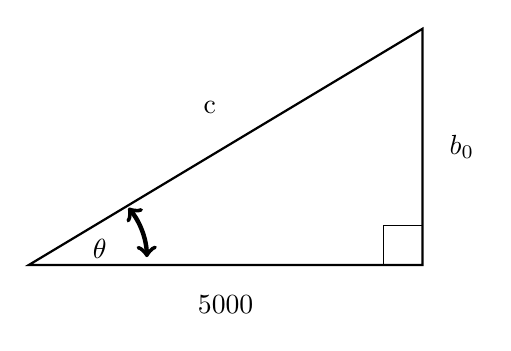
\begin{tikzpicture}
    \draw[black, thick] (0,0) -- (5,0) -- (5,3) -- cycle;
    \draw[ultra thick, <->] (1.5,.1) arc (1:40:1);
    % Below nodes are the labels.
        \node[] at (0.9, 0.2) {$\theta$};
        \node[] at (2.5, -0.5) {5000};
        \node[] at (5.5, 1.5) {$b_0$};
        \node[] at (2.3, 2) {c};
    % This draws the right angle.
        \draw(4.5,0)|-(5,.5);
\end{tikzpicture}

\bigskip

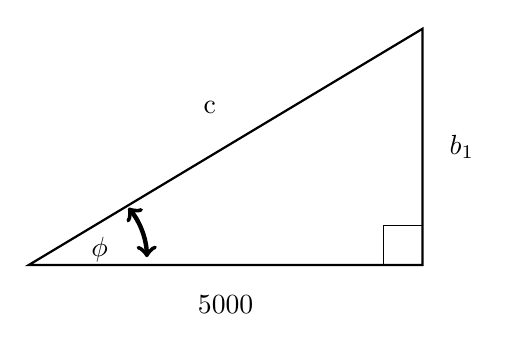
\begin{tikzpicture}
    \draw[black, thick] (0,0) -- (5,0) -- (5,3) -- cycle;
    \draw[ultra thick, <->] (1.5,.1) arc (1:40:1);
    % Below nodes are the labels.
        \node[] at (0.9, 0.2) {$\phi$};
        \node[] at (2.5, -0.5) {5000};
        \node[] at (5.5, 1.5) {$b_1$};
        \node[] at (2.3, 2) {c};
    % This draws the right angle.
        \draw(4.5,0)|-(5,.5);
\end{tikzpicture}

To solve for both heights I'll be using tangent. This makes it a cakewalk.

\[\theta = 7.970\degree\]
\[\phi = 7.125\degree\]

\bigskip

\[tan(\theta) = \frac{b_0}{5000}\]
\[\boxed{b_0 = 5000 \cdot tan(\theta)}\]

\bigskip

\[tan(\phi) = \frac{b_0}{5000}\]
\[\boxed{b_1 = 5000 \cdot tan(\phi)}\]


Now we can create a formula to calculate the distance and then just plug in our values.
\begin{align}
    x &= b_0 - b_1 \\
    x &= (5000 \cdot tan(\theta)) - (5000 \cdot tan(\phi)) \\
    x &= 5000( tan(\theta) - tan(\phi)) \\
    x &= 5000( tan(7.970\degree) - tan(7.125\degree)) \\
    x &= 700 - 625
\end{align}

\[\boxed{x = 75ft}\]
\end{solution}


\pagebreak


\begin{problem}[78a]
Show that if the horizontal is above and parallel to level ground then the angle of depression (from observer to object) and the angle of inclination (from object to observer) will be congruent because they are alternate interior angles.
\end{problem}

\begin{solution}
To solve this problem I first added a second horizontal line to the bottom of the given diagram. From there I constructed a rectangle. From there I was able to create a list of equivalencies and it really solves itself at that point. 

\bigskip 

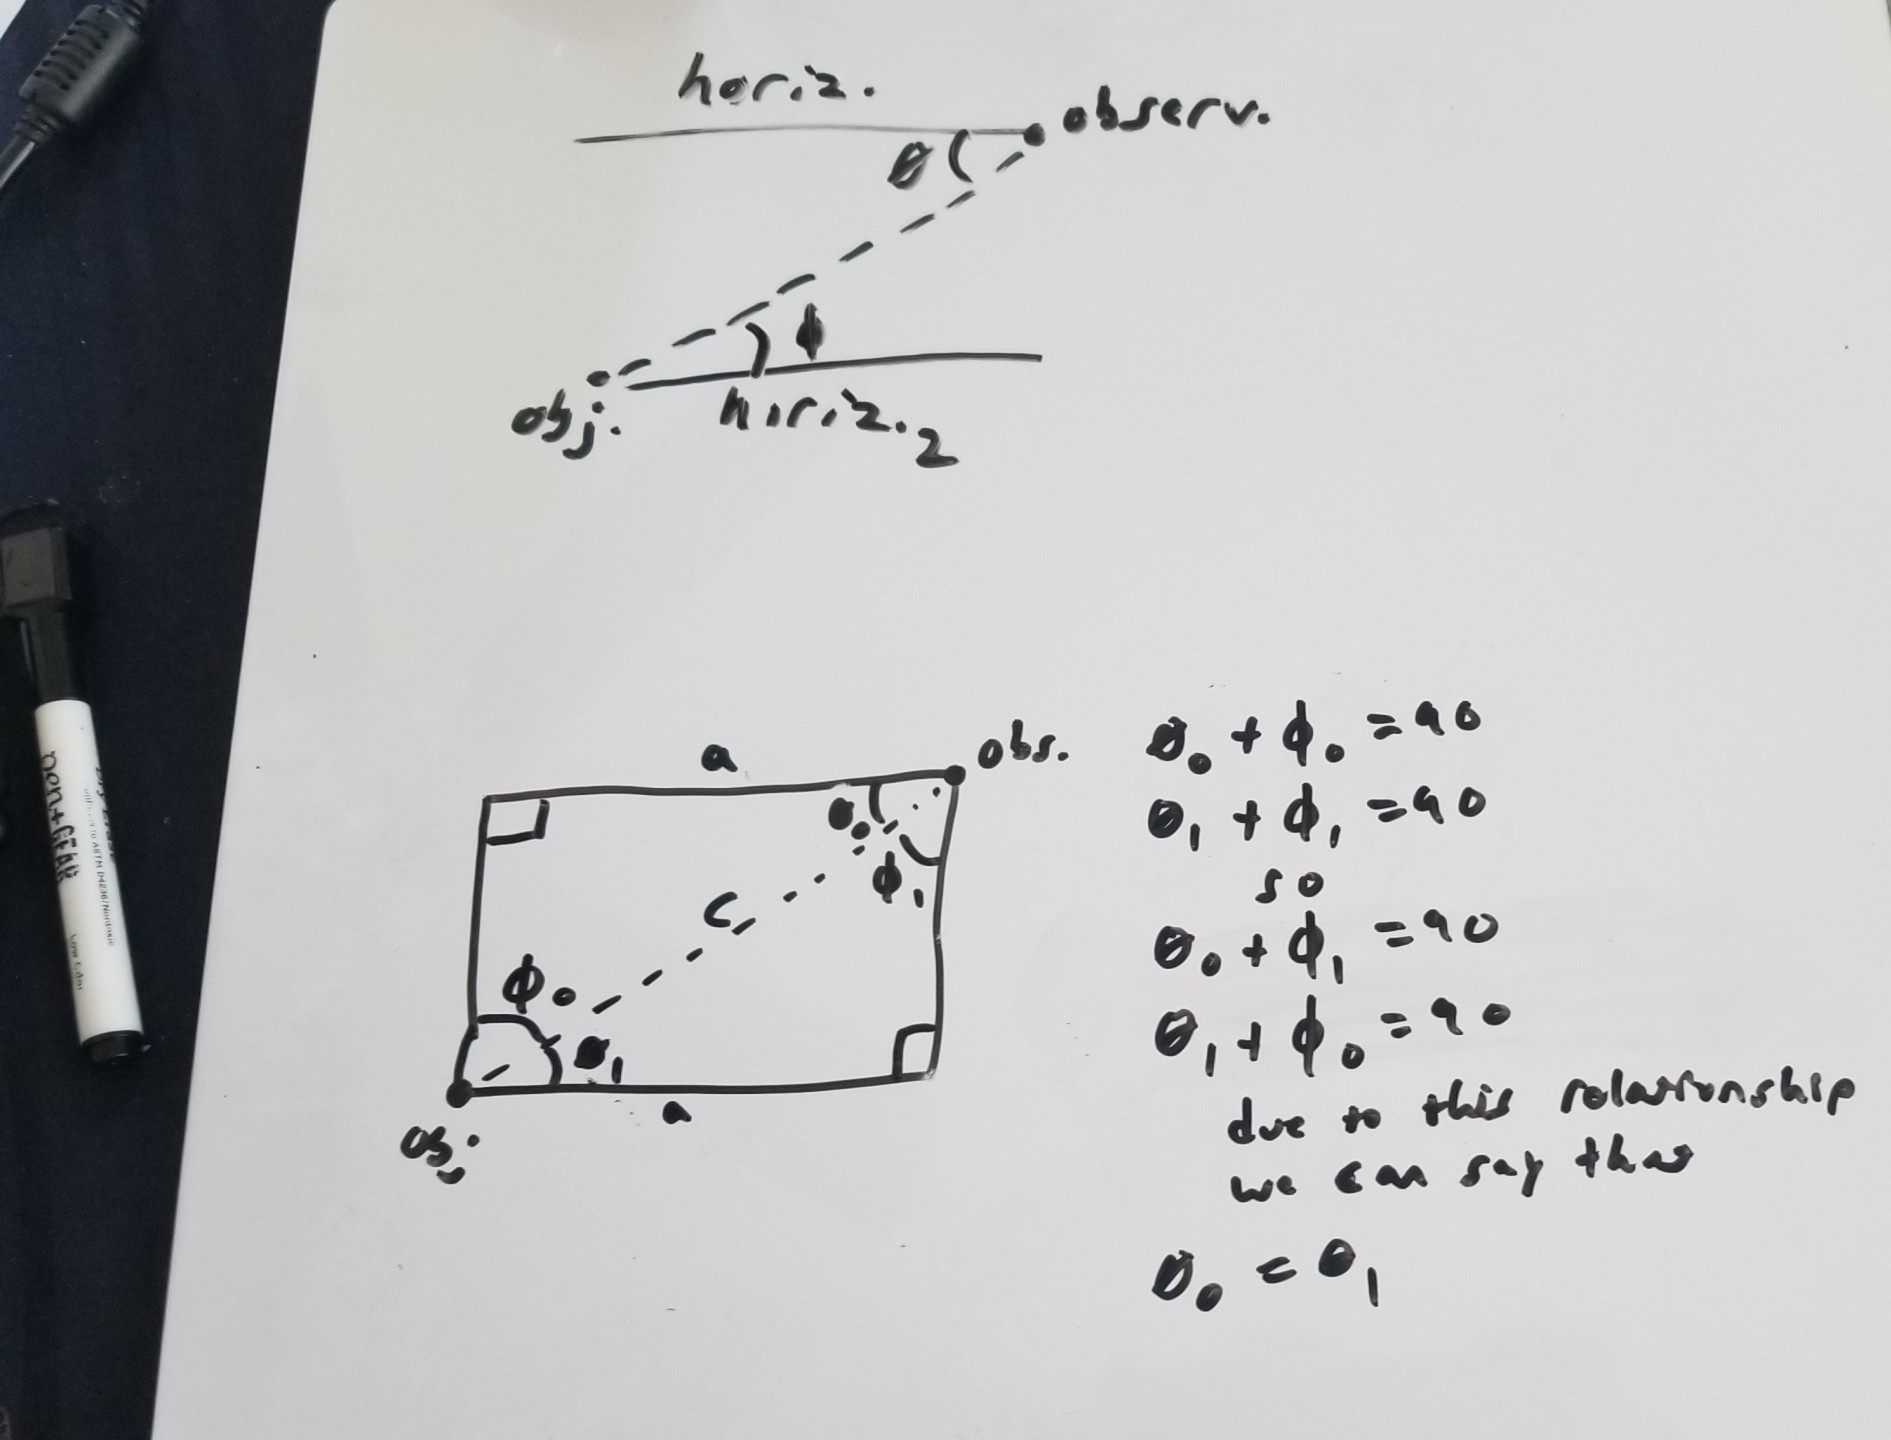
\includegraphics[width=6in,scale=1.0]{images/problem_78.jpg}
\end{solution}


\pagebreak


\begin{problem}[78b]
From a firetower 200 feet above level ground in the Sasquatch National Forest, a ranger
spots a fire off in the distance. The angle of depression to the fire is 2.5\degree. How far away
from the base of the tower is the fire?
\end{problem}

\begin{solution}

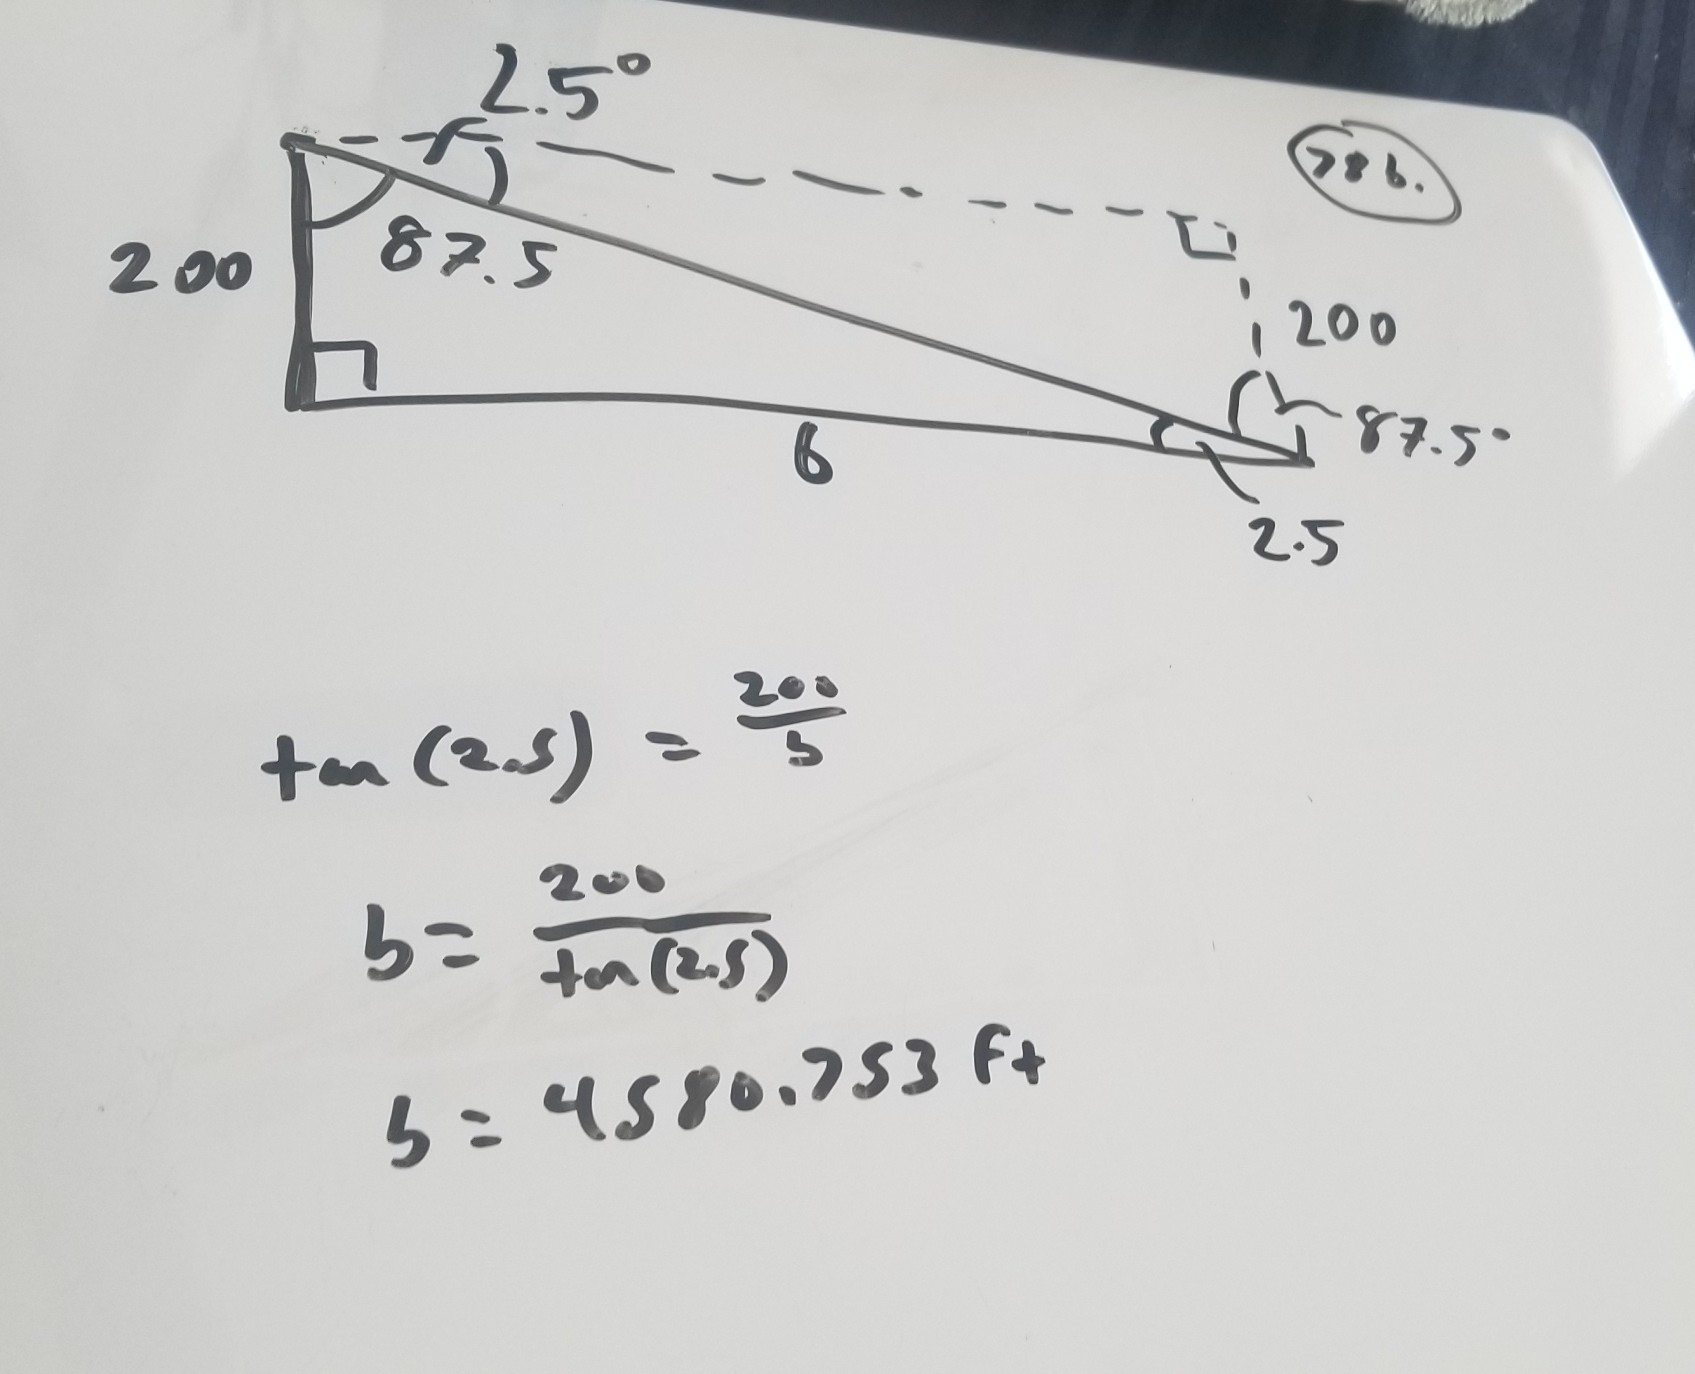
\includegraphics[width=6in, scale=1.0]{images/problem_78bb.jpg}

\end{solution}


\pagebreak


\begin{problem}[78c]
The ranger in part 78b sees a Sasquatch running directly from the fire towards the fire tower. The ranger takes two sightings. At the first sighting, the angle of depression from the tower to the Sasquatch is 6\degree. The second sighting, taken just 10 seconds later, gives the the angle of depression as 6.5\degree. How far did the Sasquatch travel in those 10 seconds? Round your answer to the nearest foot. How fast is it running in miles per hour? Round your answer to the nearest mile per hour. If the Sasquatch keeps up this pace, how long will it take for the Sasquatch to reach the fire tower from his location at the second sighting? Round your answer to the nearest minute.
\end{problem}

\begin{solution}
Take note that though the whiteboard says 78b at the top this is infact the solution to 78c. I'm just an idiot.
\bigskip

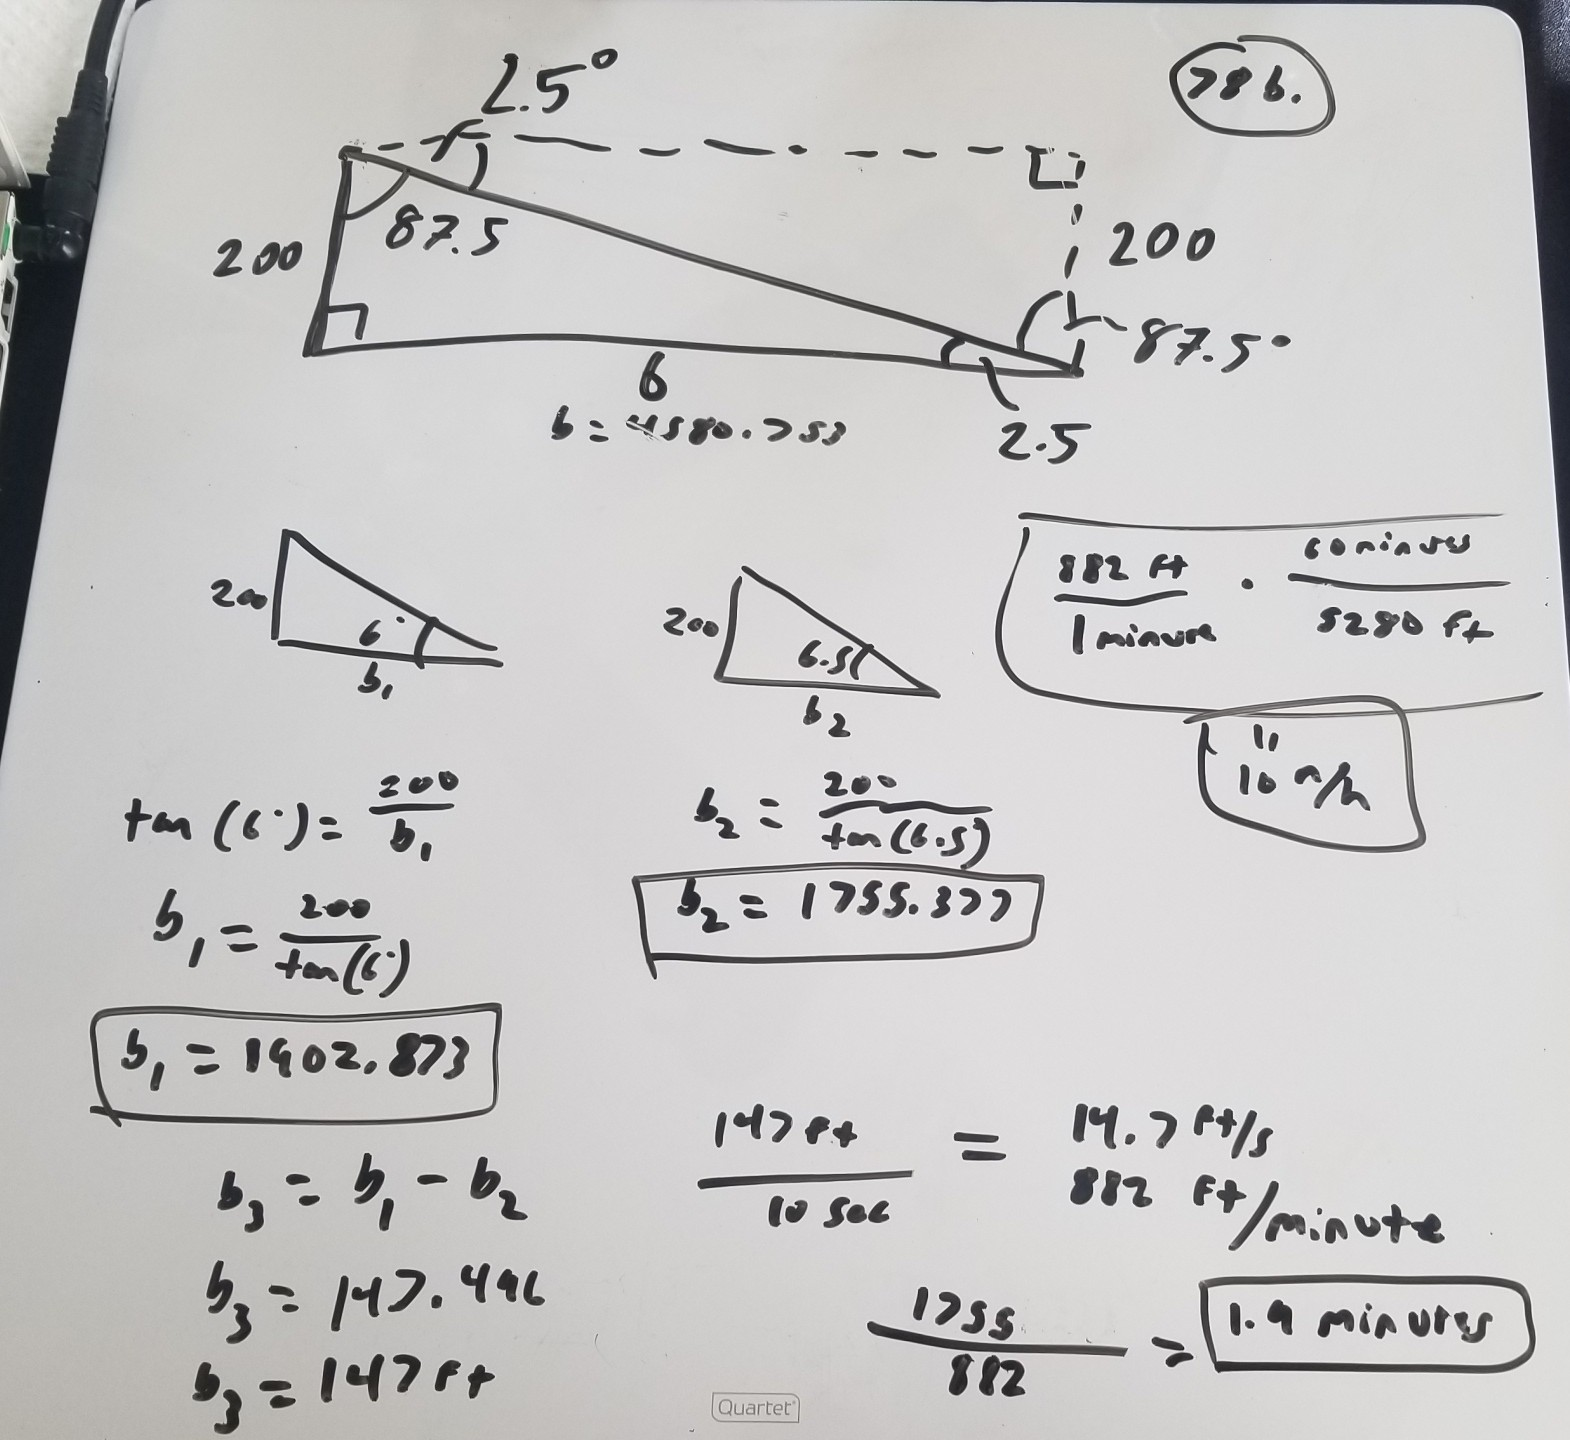
\includegraphics[width=6in, scale=1.0]{images/problem_78b.jpg}

\end{solution}


\pagebreak


\begin{problem}[79]
When I stand 30 feet away from a tree at home, the angle of elevation to the top of the tree is 50\degree and the angle of depression to the base of the tree is 10\degree. What is the height of the tree? Round your answer to the nearest foot.
\end{problem}

\begin{solution}

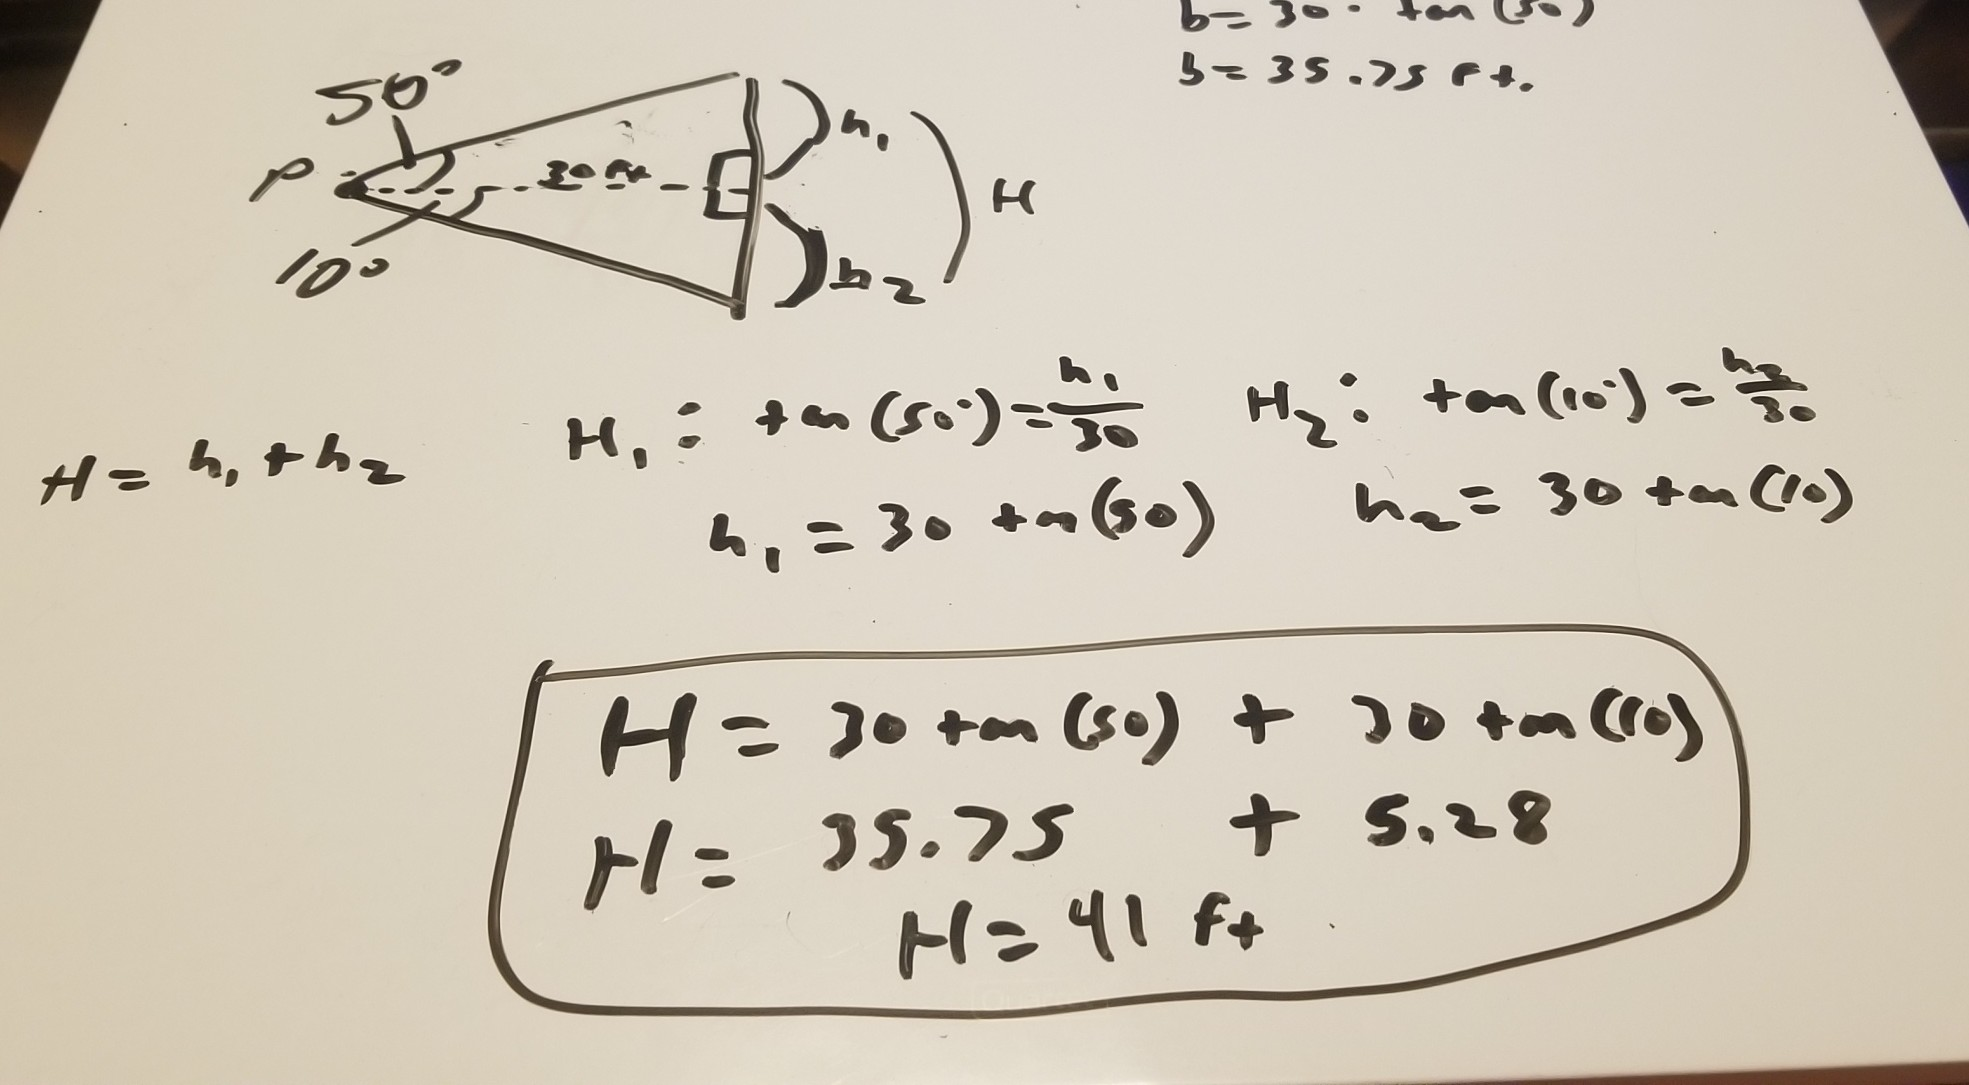
\includegraphics[width=6in, scale=1.0]{images/problem_79.jpg}

\end{solution}


\pagebreak


\begin{problem}[80]
From the observation deck of the lighthouse at Sasquatch Point 50 feet above the surface of Lake Ippizuti, a lifeguard spots a boat out on the lake sailing directly toward the lighthouse. The first sighting had an angle of depression of 8.2\degree and and the second sighting had an angle of depression of 25.9\degree. How far had the boat traveled between the sightings?
\end{problem}

\begin{solution}

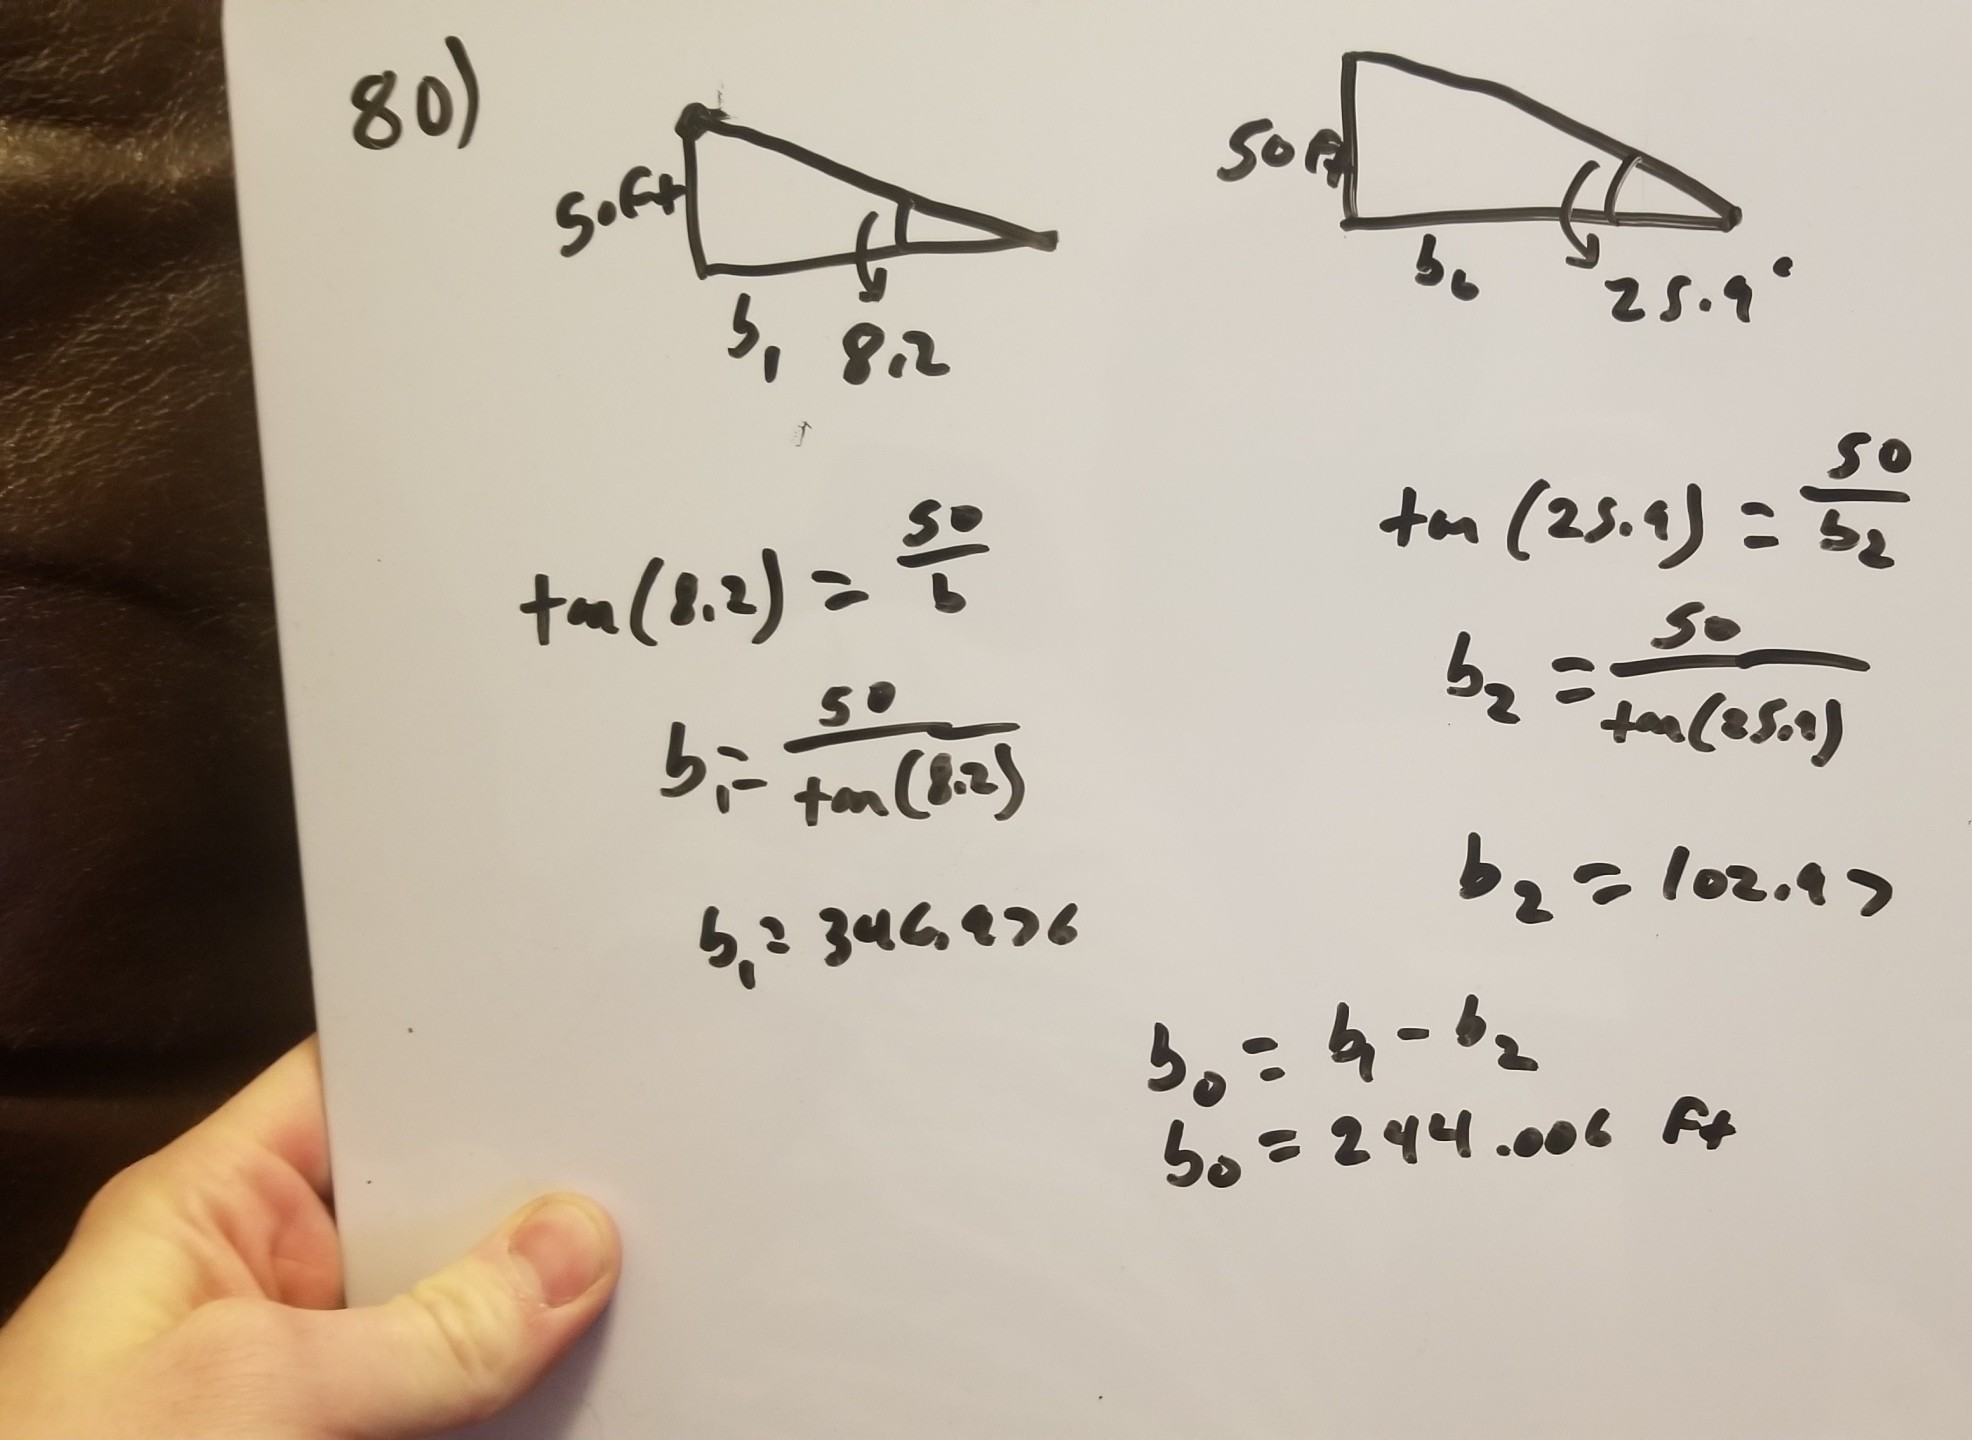
\includegraphics[width=6in, scale=1.0]{images/problem_80.jpg}

\end{solution}


\pagebreak


\begin{problem}[135]
We wish to establish the inequality $cos(\theta) < \frac{sin\theta}{\theta} < 1$ for $0 < \theta < \frac{\pi}{2}$ Use the diagram from the beginning of the section, partially reproduced below, to answer the following.

\bigskip

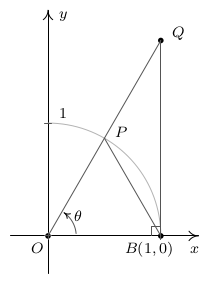
\includegraphics[width=2in, scale=1.0]{images/135_diagram.png}
\end{problem}

\begin{problem}[a]
Show that triangle OPB has area $\frac{1}{2}sin(\theta)$.
\end{problem}

\begin{solution}
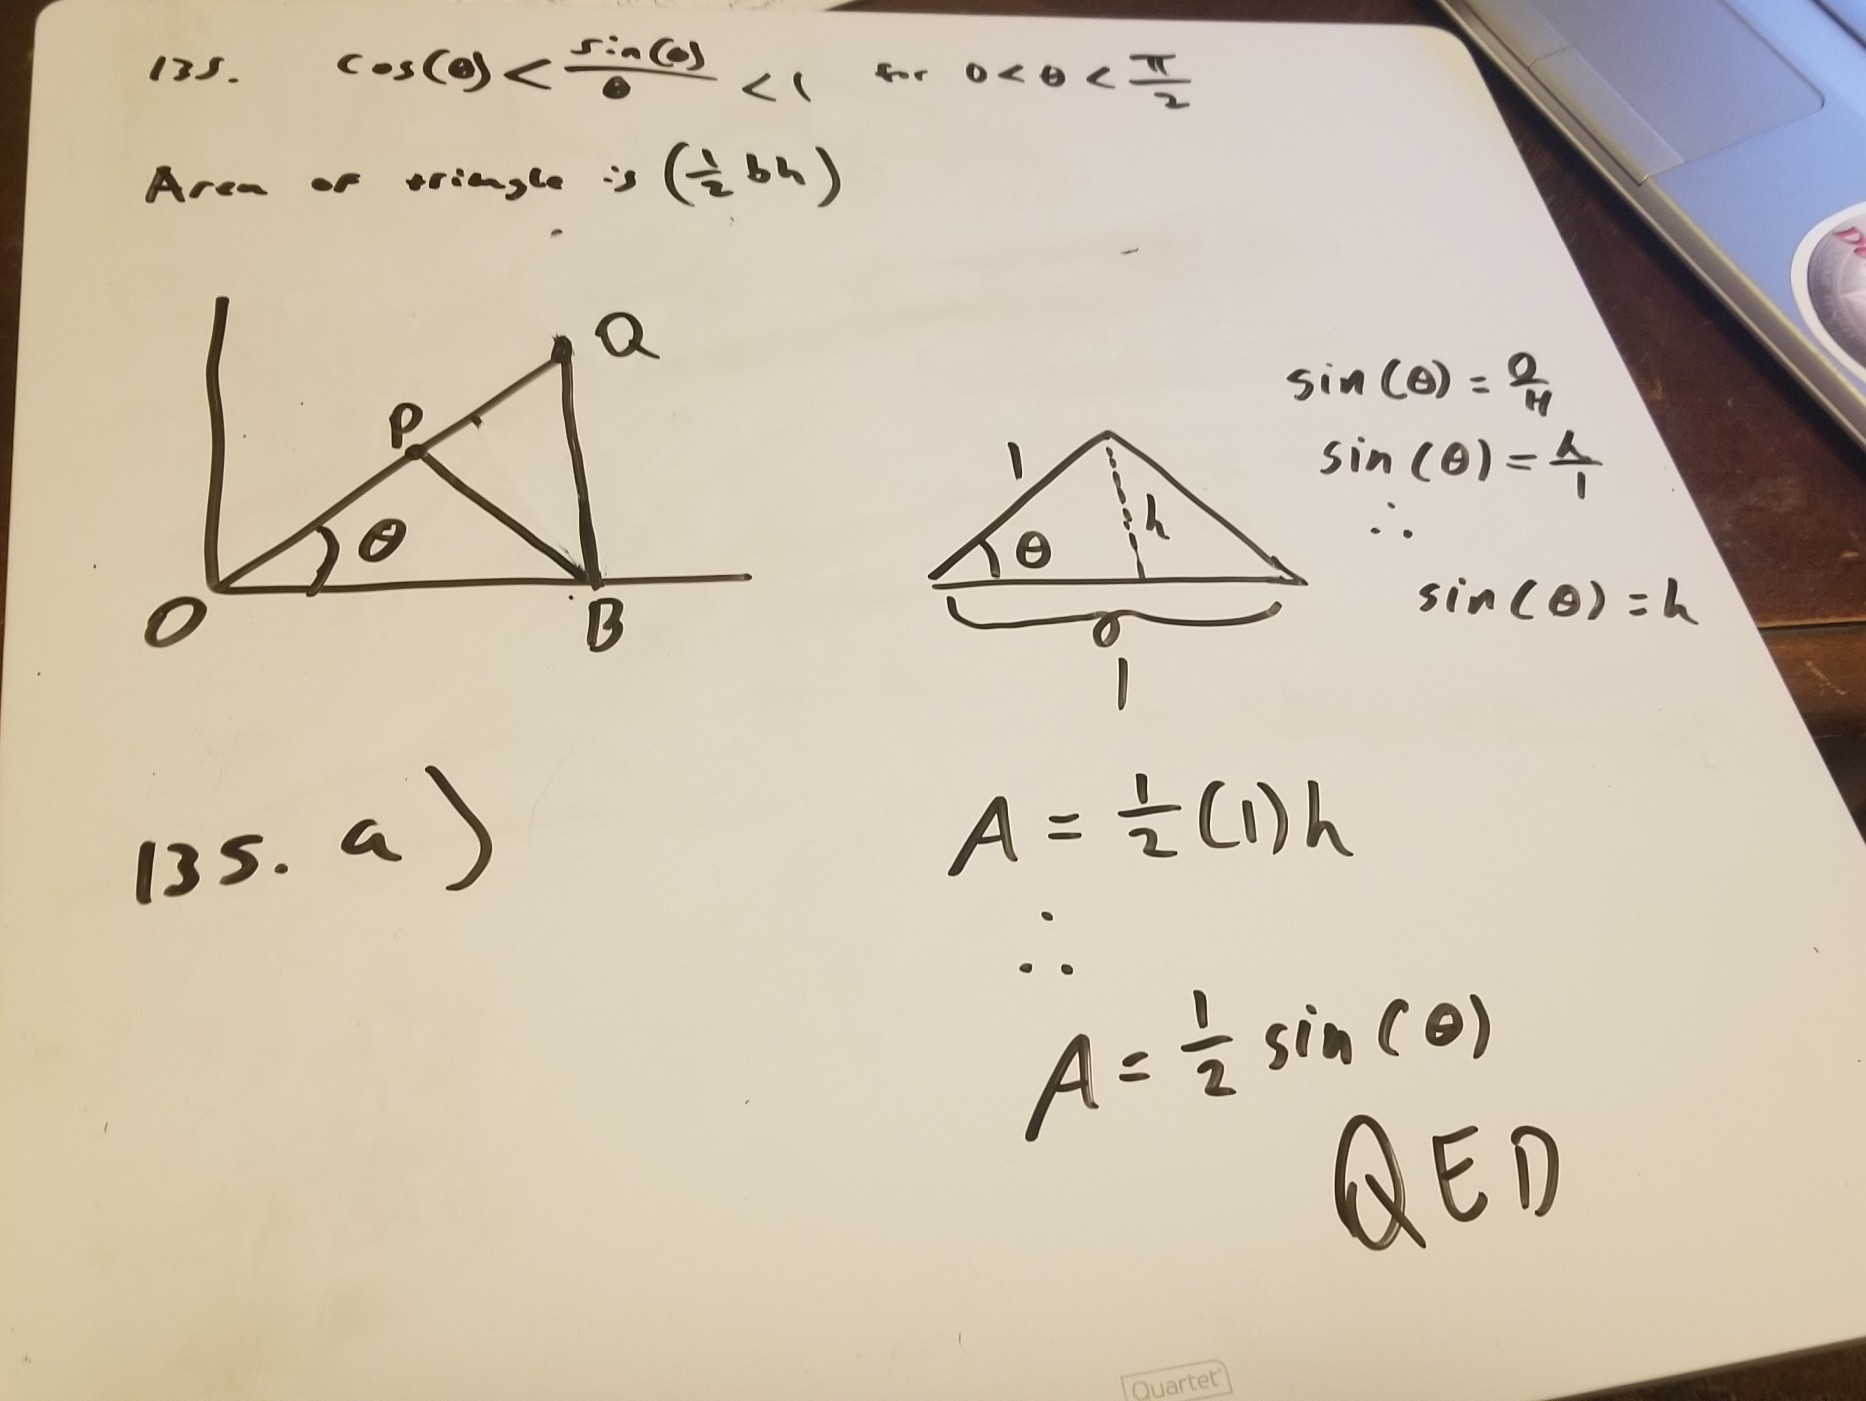
\includegraphics[width=6in, scale=1.0]{images/problem_135a.jpg}
\end{solution}

\pagebreak

\begin{problem}[b]
Show that the circular sector OPB with central angle $\theta$ has area $\frac{1}{2}\theta$.
\end{problem}

\begin{solution}
The key here is to know that the radius we're working with here is 1. 

\[A_{sector} = \frac{1}{2} r^2 \theta\]
\[A_{sector} = \frac{1}{2} (1) \theta\]
\[\boxed{A_{sector} = \frac{1}{2} \theta}\]
\end{solution}


\begin{problem}[c]
Show that triangle OQB has area $\frac{1}{2} tan(\theta)$.
\end{problem}

\begin{solution}
\begin{align}
    A_{OQB} &= \frac{1}{2}base \cdot height \\
    tan(\theta) &= \frac{h}{b} \\
    b \cdot tan(\theta) &= h \\
    A_{OQB} &= \frac{1}{2} b \cdot tan(\theta) \cdot b
\end{align}
\[\boxed{A_{OQB} = \frac{1}{2}tan(\theta)}\]
\end{solution}

\begin{problem}[d]
Comparing areas, show that $sin(\theta) < \theta < tan(\theta)$ for $0 < \theta < \frac{\pi}{2}$.
\end{problem}

\begin{solution}
\begin{align}
    A_{OBP} = \frac{1}{2} sin \theta \\
    A_{OQB} = \frac{1}{2} tan \theta \\
    A_{sector} = \frac{1}{2} \theta
\end{align}

We know:

\begin{align}
    A_{OBP} < A_{Sector} < A_{OBQ} \\
    \frac{1}{2} sin \theta < \frac{1}{2} \theta < \frac{1}{2} tan \theta \\
\end{align}

\[\boxed{sin \theta < \theta < tan \theta}\]
\begin{center}
    For $0 < \theta < \frac{\pi}{2}$
\end{center} 
\end{solution}


\pagebreak


\begin{problem}[e]
Use the inequality $sin(\theta) < \theta$ to show that $\frac{sin(\theta)}{\theta} < 1$ for $0 < \theta < \frac{\pi}{2}$.
\end{problem}

\begin{solution}
For the fraction to be less than one the numerator HAS to be smaller than the denominator. Since $sin(\theta) < \theta$ the numerator will ALWAYS be less than the denominator for $0 < \theta < \frac{\pi}{2}$.
\end{solution}


\begin{problem}[f]
Use the inequality $\theta < tan(\theta)$ to show that $cos(\theta) < \frac{sin(\theta)}{\theta}$ for $0 < \theta < \frac{\pi}{2}$.
\end{problem}

\begin{solution}
\begin{align}
    \theta &< tan(\theta) \\
    \theta &< \frac{sin(\theta)}{cos(\theta)} \\
    \theta \cdot cos(\theta) &< sin(\theta)
\end{align}
\[\boxed{cos(\theta) < \frac{sin(\theta)}{\theta}}\]
\begin{center}
    For $0 < \theta < \frac{\pi}{2}$.
\end{center}

So, now we can combine our previous conclusions together so we get the following.

\[\boxed{cos(\theta) < \frac{sin(\theta)}{\theta} < 1}\]
\begin{center}
    For $0 < \theta < \frac{\pi}{2}$
\end{center}
\end{solution}

\pagebreak


\begin{problem}[137]
Explain why the fact that $tan(\theta) = 3 = \frac{3}{1}$ does not mean $sin(\theta) = 3$ and $cos(\theta) = 1$?
\end{problem}

\begin{solution}
I think there are a few things we can point out. Firstly, all of these trigonometric functions are ratios. Let's look at this for instance.

\[x = \frac{a}{b}\]
\[x = 6 = \frac{6}{1}\]
This doesn't mean that a has to equal 6 or that b has to equal one. We could have something like this.
\[x = \frac{1200}{200}\]
This satisfies those requirements without a being 6 or b being 1. It's a ratio. What that means is there are an infinite number of solutions that could meet those requirements. It's also important to take note of the ranges of sine and cosine when compared to tangent. Sine and cosine both have a range of $-1 \leq \theta \leq 1$. Tangent meanwhile has a range of all real numbers ($\mathbb{R}$).

\end{solution}

\pagebreak
\centering \textbf{References}     


Figure 1.
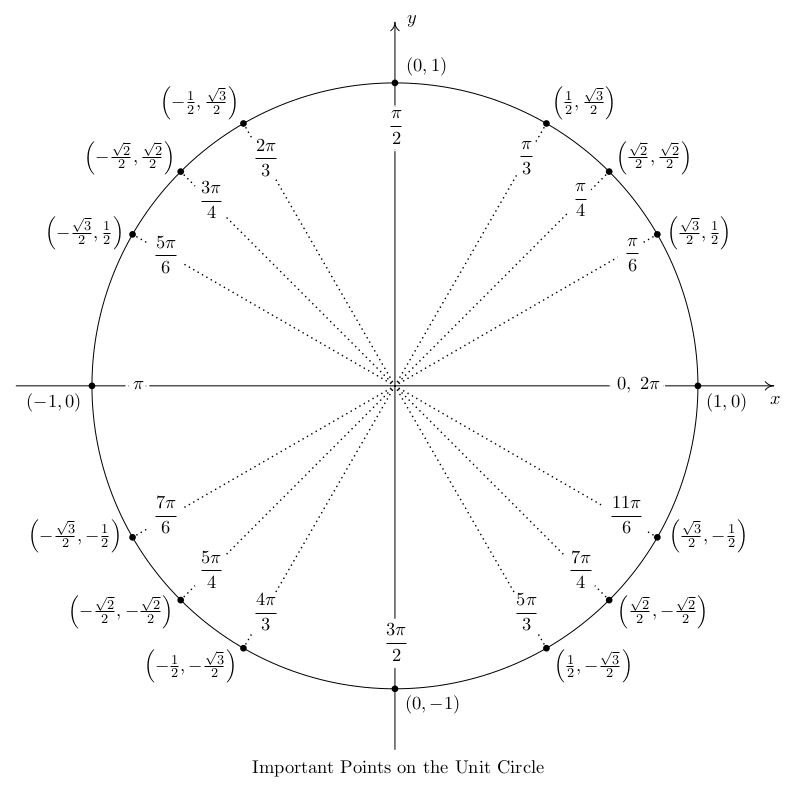
\includegraphics[width=6in,scale=1.0]{images/unit_circle.png}

Figure 2.
\begin{center}
\begin{tabular}{ |c|c|c|c|c| } 
 \hline
  $\theta$(degrees) & $\theta$(radians) & cos($\theta$) & sin ($\theta$) & tan ($\theta$) \\ [1.0ex] 
 \hline\hline
 0\degree & 0 & 1 & 0 & 0\\[+3mm] 
 \hline
 $30\degree$ & $\frac{\pi}{2}$ & $\frac{\sqrt{2}}{2}$ & $\frac{1}{2}$ & $\frac{1}{\sqrt{3}}$\\[+3mm] 
 \hline
 $45\degree$ & $\frac{\pi}{4}$ & $\frac{\sqrt{2}}{2}$ & $\frac{\sqrt{2}}{2}$ & 1\\[+3mm]
 \hline
 $60\degree$ & $\frac{\pi}{3}$ & $\frac{1}{2}$ & $\frac{\sqrt{3}}{2}$ & $\sqrt{3}$ \\[+3mm]
 \hline
 $90\degree$ & $\frac{\pi}{2}$ & 0 & 1 & inf\\
 \hline
\end{tabular}
\end{center}
\end{document}
